\section{Network configuration}
The network configuration utility is accessed by the front page of the Morfeas WEB from the button with
this 
\includegraphics[height=.125in]{../art/eth.png} symbol.
At figure \ref{fig:net_conf} shown an example of the network configuration utility.

\begin{figure}[h]
\centering
	\fbox{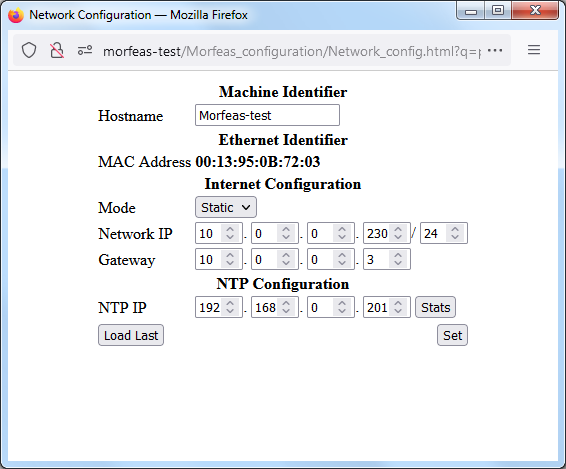
\includegraphics[width=2.5in,angle=0]{../art/Morfeas_web_if/network_config.png}}
	\caption{Morfeas WEB Utility for Network Configuration}
	\label{fig:net_conf}
\end{figure}

\begin{table}[h!]
	\begin{center}
		\begin{tabular}{|c|l|}
			\hline
			\textbf{Value} & \textbf{Purpose}\\
			\hline
			Hostname & Name for discovery services (avahi, samba, etc)\\
			\hline
			MAC Address & Identifier of the Ethernet interface\\
			\hline
			Mode & Internet address configuration mode (Static, DHCP)\\
			\hline
			Network IP & IP address and subnet range bits (In static mode only)\\
			Gateway & Gateway's IP address (In static mode only)\\
			\hline
			NTP IP & IP address of the local network time protocol server\\
			\hline
			SDAQNet(CAN-ifs) & Configuration of the bitrate for each available can-if\\
			\hline
		\end{tabular}
		\caption{Network configuration values}
		\label{tab:net_conf}
	\end{center}
\end{table}

At table \ref{tab:net_conf} present the values and purpose of the configuration fields of the utility.
The two buttons at the bottom of the utility window(Load last, Set),
have purpose to send the current configuration to the device (Set),
and reload the last configuration from the device (Load Last).